\documentclass[12pt, a4paper]{article}
\usepackage[utf8]{inputenc}
\usepackage[russian]{babel}
\usepackage[pdftex]{graphicx, color}
\usepackage[left=2cm,right=2cm,top=1.5cm,bottom=2cm]{geometry}
\usepackage{indentfirst}
\usepackage{hyperref}
\usepackage[justification=centering,labelfont=bf]{caption, subcaption}
\usepackage{amsmath, amsfonts, amssymb, amsthm, amsbsy, mathtools}
\usepackage{mdframed}
\usepackage{setspace}
\usepackage{enumitem}
\usepackage[table,xcdraw]{xcolor}
\usepackage{multirow}
\usepackage{float}

% \onehalfspacing

\title{
    
\includegraphics[height=3cm]{pics/msu.png} \\
    \large{
        Результаты запусков программ \textbf{jac} и \textbf{mgrid}
    }
}
\author{
    \normalsize{Аят Оспанов} \\
    \normalsize{617 группа, ММП, ВМК МГУ, Москва}
}
\date{\normalsize{11 декабря 2017 г.}}

\begin{document}
    \maketitle
    \tableofcontents

    \section{Ускорение}
        \begin{table}[H]
        \centering
        \caption{Ускорение программы jac}
        \label{tab:jac}
        \begin{tabular}{llll
        >{\columncolor[HTML]{EFEFEF}}l
        >{\columncolor[HTML]{EFEFEF}}l }
        \cellcolor[HTML]{C0C0C0}                                                                                                           & \multicolumn{3}{c}{\cellcolor[HTML]{C0C0C0}\textbf{Время работы, сек}}                                                                                               & \multicolumn{2}{c}{\cellcolor[HTML]{C0C0C0}\textbf{Ускорение}}                                         \\
        \multirow{-2}{*}{\cellcolor[HTML]{C0C0C0}\textbf{\begin{tabular}[c]{@{}l@{}}Размер сетки\\ $N \times 400 \times 50$\end{tabular}}} & \cellcolor[HTML]{C0C0C0}{\color[HTML]{000000} \textbf{CPU}} & \cellcolor[HTML]{C0C0C0}{\color[HTML]{000000} \textbf{1 GPU}} & \cellcolor[HTML]{C0C0C0}\textbf{2 GPU} & \cellcolor[HTML]{C0C0C0}{\color[HTML]{000000} \textbf{1 GPU}} & \cellcolor[HTML]{C0C0C0}\textbf{2 GPU} \\
        500                                                                                                                                & 26.25                                                       & 1.88                                                          & 1.02                                   & 13.96                                                         & 25.74                                  \\
        700                                                                                                                                & 36.68                                                       & 2.61                                                          & 1.43                                   & 14.05                                                         & 25.65                                  \\
        900                                                                                                                                & 47.49                                                       & 3.35                                                          & 1.81                                   & 14.17                                                         & 26.24                                  \\
        1100                                                                                                                               & 57.65                                                       & 4.09                                                          & 2.21                                   & 14.10                                                         & 26.09                                  \\
        1300                                                                                                                               & 68.90                                                       & 4.83                                                          & 2.61                                   & 14.27                                                         & 26.40                                  \\
        1500                                                                                                                               & 79.61                                                       & 5.57                                                          & 3.00                                   & 14.29                                                         & 26.54                                  \\
        1700                                                                                                                               & 89.64                                                       & 6.30                                                          & 3.38                                   & 14.23                                                         & 26.52
        \end{tabular}
        \end{table}

        Таблица \ref{tab:jac} была построена для размера блока $32\times32$. Но в данном случае, occupancy будет не 100\%. Т.к. на тестируемой машине установлена видеокарта GTX 550 Ti, то ее характеристики следующие:
        \begin{itemize}
            \item Максимальное количество нитей на мультипроцессор -- 1536
            \item Максимальное количество нитей на блок -- 1024
            \item Максимальное количество блоков на мультипроцессор -- 8
        \end{itemize}

        Таким образом, если размер блока $32\times32$, то нитей в блоке $32 * 32 = 1024$, а блоков $1$ и occupancy = $1024 * 1 / 1536 = 66\%$. Чтобы ускорить программу, было решено взять два разных размера блоков, таким образом, что occupancy = $100\%$: $32\times16$ и $16\times16$ ($32 * 16 * 3 / 1536 = 16 * 16 * 6 / 1536 = 100\%$)

        \begin{table}[H]
        \centering
        \caption{Ускорение программы jac в зависимости от размера блока}
        \label{tab:jac_grid}
        \begin{tabular}{llll
        >{\columncolor[HTML]{EFEFEF}}l
        >{\columncolor[HTML]{EFEFEF}}l }
        \cellcolor[HTML]{C0C0C0}                                                                                                           & \multicolumn{3}{l}{\cellcolor[HTML]{C0C0C0}\textbf{Время работы на 2 GPU, сек}}                                                                 & \multicolumn{2}{l}{\cellcolor[HTML]{C0C0C0}\textbf{Ускорение}}                  \\
        \multirow{-2}{*}{\cellcolor[HTML]{C0C0C0}\textbf{\begin{tabular}[c]{@{}l@{}}Размер сетки\\ $N \times 400 \times 50$\end{tabular}}} & \cellcolor[HTML]{C0C0C0}{\color[HTML]{000000} \textbf{32x32}} & \cellcolor[HTML]{C0C0C0}\textbf{32x16} & \cellcolor[HTML]{C0C0C0}\textbf{16x16} & \cellcolor[HTML]{C0C0C0}\textbf{32x16} & \cellcolor[HTML]{C0C0C0}\textbf{16x16} \\
        500                                                                                                                                & 1.02                                                          & 0.88                                   & 0.83                                   & 1.16                                   & 1.23                                   \\
        700                                                                                                                                & 1.43                                                          & 1.21                                   & 1.12                                   & 1.18                                   & 1.28                                   \\
        900                                                                                                                                & 1.81                                                          & 1.54                                   & 1.43                                   & 1.18                                   & 1.27                                   \\
        1100                                                                                                                               & 2.21                                                          & 1.87                                   & 1.73                                   & 1.18                                   & 1.28                                   \\
        1300                                                                                                                               & 2.61                                                          & 2.21                                   & 2.01                                   & 1.18                                   & 1.30                                   \\
        1500                                                                                                                               & 3.00                                                          & 2.54                                   & 2.31                                   & 1.18                                   & 1.30                                   \\
        1700                                                                                                                               & 3.38                                                          & 2.87                                   & 2.68                                   & 1.18                                   & 1.26
        \end{tabular}
        \end{table}

        Из таблицы явно видно, что в обоих случаях есть ускорение, но для сетки $16\times16$ ускорение на $10\%$ больше. В итоге правильным подбором размера сетки мы ускорили программу на $\approx30\%$

        \begin{figure}[H]
            \caption{Программа jac}
            \label{fig:jac}
            \centering
            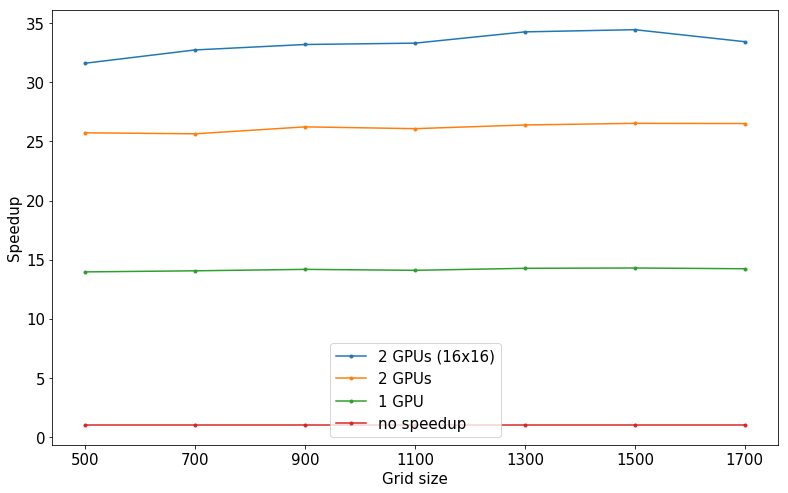
\includegraphics[width=0.8\textwidth]{pics/jac}
        \end{figure}

        Для программы mgrid ситуация примерно такая же.

        \begin{table}[H]
        \centering
        \caption{Ускорение программы mgrid}
        \label{tab:mgrid}
        \begin{tabular}{llll
        >{\columncolor[HTML]{EFEFEF}}l
        >{\columncolor[HTML]{EFEFEF}}l }
        \cellcolor[HTML]{C0C0C0}                                                                                                           & \multicolumn{3}{c}{\cellcolor[HTML]{C0C0C0}\textbf{Время работы, сек}}                                                                                               & \multicolumn{2}{c}{\cellcolor[HTML]{C0C0C0}\textbf{Ускорение}}                                         \\
        \multirow{-2}{*}{\cellcolor[HTML]{C0C0C0}\textbf{\begin{tabular}[c]{@{}l@{}}Размер сетки\\ $N \times 400 \times 50$\end{tabular}}} & \cellcolor[HTML]{C0C0C0}{\color[HTML]{000000} \textbf{CPU}} & \cellcolor[HTML]{C0C0C0}{\color[HTML]{000000} \textbf{1 GPU}} & \cellcolor[HTML]{C0C0C0}\textbf{2 GPU} & \cellcolor[HTML]{C0C0C0}{\color[HTML]{000000} \textbf{1 GPU}} & \cellcolor[HTML]{C0C0C0}\textbf{2 GPU} \\
        500                                                                                                                                & 34.84                                                       & 3.03                                                          & 1.98                                   & 11.50                                                         & 17.60                                  \\
        700                                                                                                                                & 48.77                                                       & 4.06                                                          & 2.52                                   & 12.01                                                         & 19.35                                  \\
        900                                                                                                                                & 62.73                                                       & 5.07                                                          & 3.09                                   & 12.37                                                         & 20.30                                  \\
        1100                                                                                                                               & 76.71                                                       & 6.09                                                          & 3.65                                   & 12.60                                                         & 21.02                                  \\
        1300                                                                                                                               & 90.66                                                       & 7.29                                                          & 4.20                                   & 12.44                                                         & 21.59                                  \\
        1500                                                                                                                               & 104.70                                                      & 8.56                                                          & 4.78                                   & 12.23                                                         & 21.90                                  \\
        1700                                                                                                                               & 118.66                                                      & 9.88                                                          & 5.56                                   & 12.01                                                         & 21.34
        \end{tabular}
        \end{table}

        \begin{table}[H]
        \centering
        \caption{Ускорение программы mgrid в зависимости от размера блока}
        \label{tab:mgrid_grid}
        \begin{tabular}{llll
        >{\columncolor[HTML]{EFEFEF}}l
        >{\columncolor[HTML]{EFEFEF}}l }
        \cellcolor[HTML]{C0C0C0}                                                                                                           & \multicolumn{3}{l}{\cellcolor[HTML]{C0C0C0}\textbf{Время работы на 2 GPU, сек}}                                                                 & \multicolumn{2}{l}{\cellcolor[HTML]{C0C0C0}\textbf{Ускорение}}                  \\
        \multirow{-2}{*}{\cellcolor[HTML]{C0C0C0}\textbf{\begin{tabular}[c]{@{}l@{}}Размер сетки\\ $N \times 400 \times 50$\end{tabular}}} & \cellcolor[HTML]{C0C0C0}{\color[HTML]{000000} \textbf{32x32}} & \cellcolor[HTML]{C0C0C0}\textbf{32x16} & \cellcolor[HTML]{C0C0C0}\textbf{16x16} & \cellcolor[HTML]{C0C0C0}\textbf{32x16} & \cellcolor[HTML]{C0C0C0}\textbf{16x16} \\
        500                                                                                                                                & 1.98                                                          & 1.79                                   & 1.65                                   & 1.11                                   & 1.20                                   \\
        700                                                                                                                                & 2.52                                                          & 2.26                                   & 2.07                                   & 1.12                                   & 1.22                                   \\
        900                                                                                                                                & 3.09                                                          & 2.76                                   & 2.49                                   & 1.12                                   & 1.24                                   \\
        1100                                                                                                                               & 3.65                                                          & 3.24                                   & 2.94                                   & 1.13                                   & 1.24                                   \\
        1300                                                                                                                               & 4.20                                                          & 3.73                                   & 3.38                                   & 1.13                                   & 1.24                                   \\
        1500                                                                                                                               & 4.78                                                          & 4.23                                   & 3.81                                   & 1.13                                   & 1.25                                   \\
        1700                                                                                                                               & 5.56                                                          & 4.94                                   & 4.47                                   & 1.13                                   & 1.24
        \end{tabular}
        \end{table}

        \begin{figure}[H]
            \caption{Программа mgrid}
            \label{fig:mgrid}
            \centering
            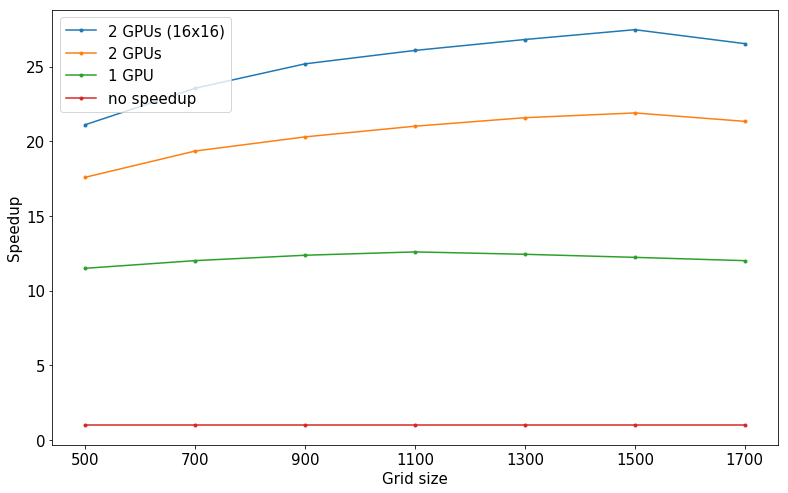
\includegraphics[width=0.8\textwidth]{pics/mgrid}
        \end{figure}

    \section{Профилировка}
        Профилировки для программ для наглядности были сделаны на 10 итерациях.

        По скриншоту профилировки программы jac (Рис. \ref{fig:prof_jac}) видно, что основное время (93\%) работы программы (не считая работу с данными) занимает работа основного ядра (\verb|jac_kernel|). Также видно (Рис. \ref{fig:prof_jac_zoomed}), что две карты работают одновременно, что подтверждает правильность реализации на двух GPU. Таким образом, программа распараллелена макимально.

        \begin{figure}[H]
            \centering
            \caption{Профилировка программы jac (мелкий план)}
            \label{fig:prof_jac}
            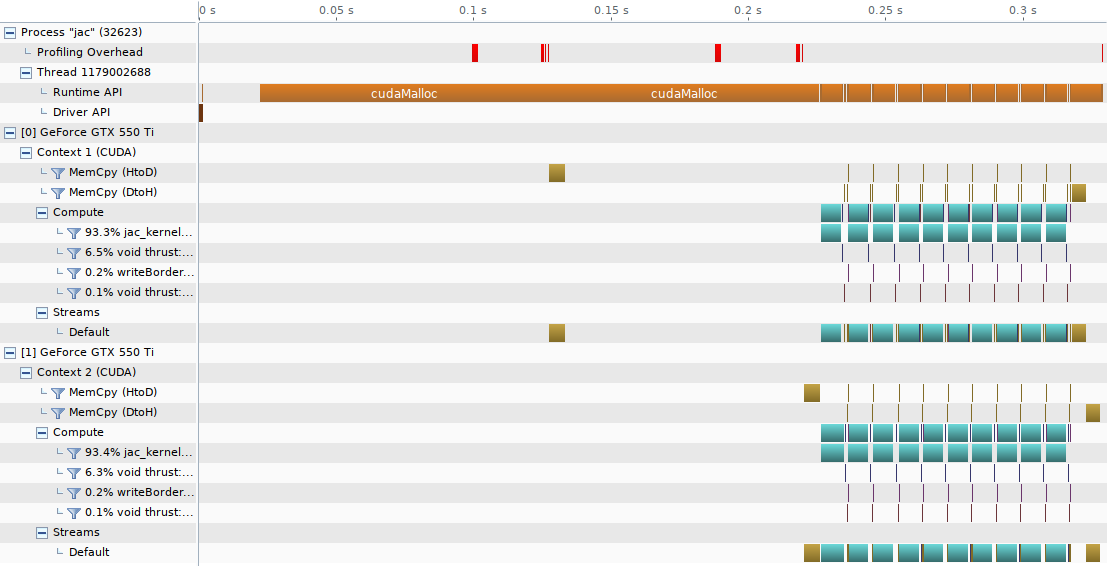
\includegraphics[width=\textwidth]{pics/prof_jac}
        \end{figure}
        \begin{figure}[H]
            \centering
            \caption{Профилировка программы jac (крупный план)}
            \label{fig:prof_jac_zoomed}
            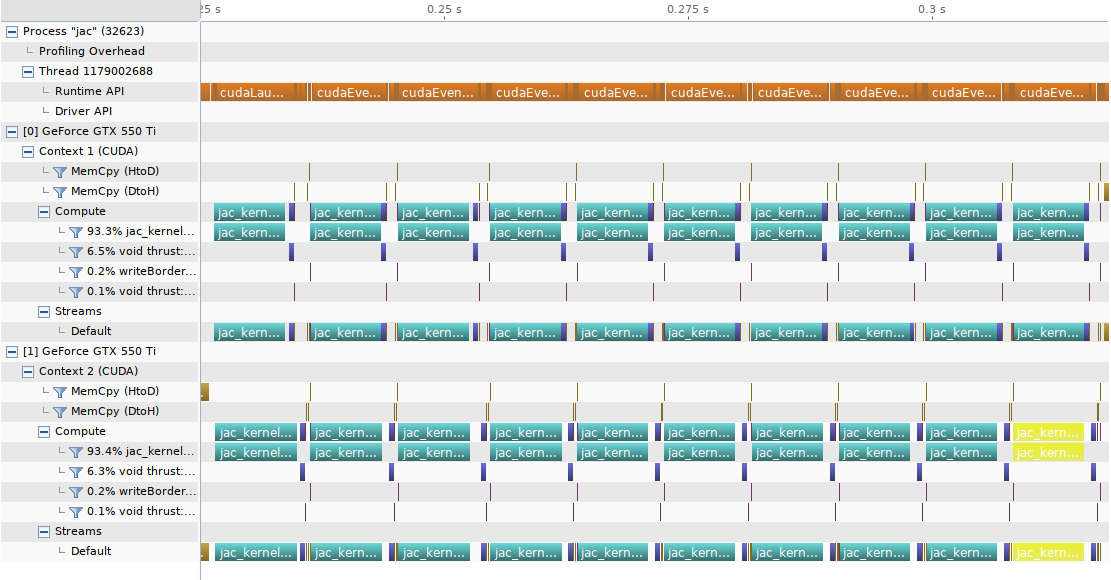
\includegraphics[width=\textwidth]{pics/prof_jac_zoomed}
        \end{figure}

        В случае mgrid можно видеть много мелких вызовов. Это вызовы ядер на измельченных данных вызываемые в рекурсии. Поэтому рассмотрим основной цикл (Рис. \ref{fig:prof_mgrid_zoomed}). В таком увеличении видно, что программа работает аналогично jac. Таким образом можно сделать вывод, что программа полностью распараллелена.

        \begin{figure}[H]
            \centering
            \caption{Профилировка программы mgrid (мелкий план)}
            \label{fig:prof_mgrid}
            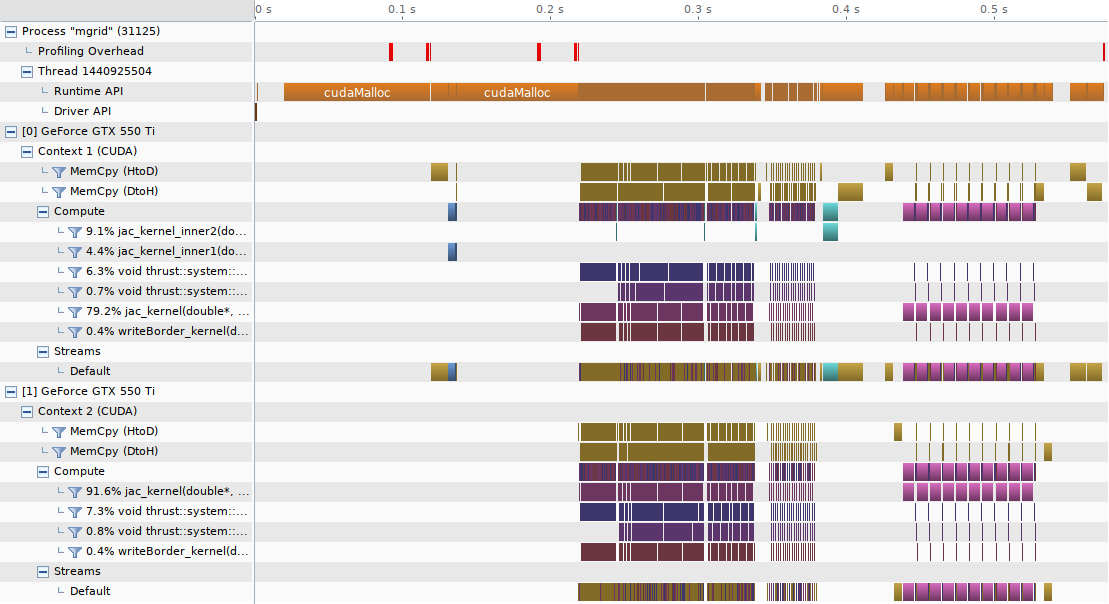
\includegraphics[width=\textwidth]{pics/prof_mgrid}
        \end{figure}
        \begin{figure}[H]
            \centering
            \caption{Профилировка программы mgrid (крупный план)}
            \label{fig:prof_mgrid_zoomed}
            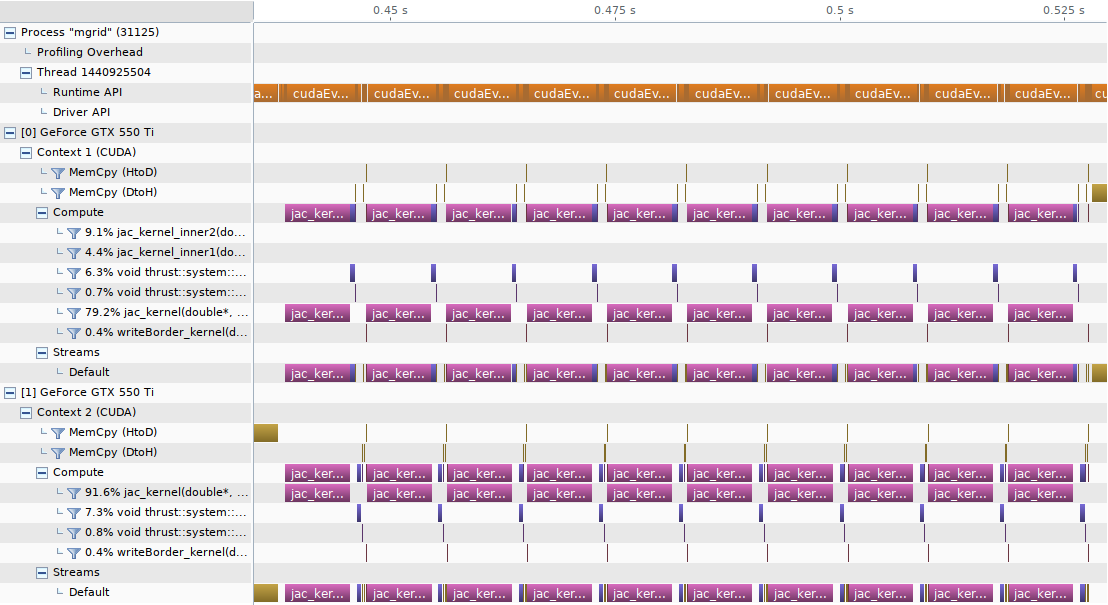
\includegraphics[width=\textwidth]{pics/prof_mgrid_zoomed}
        \end{figure}

\end{document}
